%!TEX TS-program = xelatex
\documentclass[a4paper,14pt]{extarticle}
\usepackage{geometry}
\geometry{
    a4paper,
    top=20mm,
    bottom=20mm,
    left=30mm,    % ГОСТ: левое поле 30 мм
    right=15mm,   % правое поле 15 мм
    bindingoffset=0mm
}

\usepackage{fontspec}
\usepackage{graphicx}
\usepackage{enumitem}
\usepackage{multicol}
\usepackage[hidelinks]{hyperref}
\usepackage{soul} % для выделения текста
\usepackage{minted}
\usepackage{lipsum}
\usepackage{indentfirst}
\usepackage[labelsep=endash]{caption}
\usepackage{titlesec} % Пакет для настройки заголовков
\usepackage{pgfplots}
\usepackage{mwe}
\usepackage{polyglossia} % Для поддержки русского языка
\usepackage{tabularx}
\usepackage{longtable}
\usepackage{booktabs}
\usepackage{float}
\usepackage{csquotes}

\usepackage{polyglossia}
\setmainlanguage{russian}  % ← Основной язык
\setotherlanguage{english} % ← Дополнительный 
% \usepackage[english, russian]{babel}

% Шрифт TeX Gyre Termes вместо Times New Roman но все ещё по ГОСТ
\usepackage{fontspec}
\setmainfont{PT Serif}[
  Language=Russian,
  Script=Cyrillic
]
% \setmainfont{Times New Roman}


% Межстрочный интервал 1.5 по ГОСТ
\usepackage{setspace}
\onehalfspacing

% Отступ первой строки абзаца 1.25 см
\usepackage{indentfirst}
\setlength{\parindent}{1.25cm}

% Настройка заголовков по ГОСТ
\usepackage{titlesec}
\titleformat{\section}{\normalsize\bfseries\centering}{\thesection}{1em}{}
\titleformat{\subsection}{\normalsize\bfseries\centering}{\thesubsection}{1em}{}
\titlespacing*{\section}{0pt}{12pt}{12pt}  % Отступы вокруг заголовков

% Настройка переносов через polyglossia
\PolyglossiaSetup{russian}{
    hyphenmins = {2,3}, % мин. 2 символа до и 3 после переноса
    spelling = modern,
    hyphenation = { % Аналог babelhyphenation
        про-из-во-ди-тель-ность,
        PostgreSQL,
        мас-шта-би-ро-ва-ние
    }
}

\addto\captionsrussian{\renewcommand{\contentsname}{СОДЕРЖАНИЕ}}
\usepackage{tocloft}
\renewcommand{\cftsecleader}{\cftdotfill{\cftdotsep}}

\usepackage{array} % Для настройки таблиц
\newcolumntype{L}[1]{>{\raggedright\let\newline\\\arraybackslash\hspace{0pt}}p{#1}}
\newcolumntype{C}[1]{>{\centering\let\newline\\\arraybackslash\hspace{0pt}}p{#1}}
\newcolumntype{L}[1]{>{\raggedright\arraybackslash}p{#1}}

\newcommand{\red}[1]{\textcolor{red}{#1}} % для разметки 

\definecolor{markerlightyellow}{RGB}{255,255,200} 
\sethlcolor{markerlightyellow} % установка цвета выделени

\usepackage[
    backend=biber,
    style=gost-numeric,  % Стиль ГОСТ (нумерованный)
    sorting=none,        % Сортировка в порядке упоминания
    language=auto,       % Автоматическое определение языка
    autolang=other,      % Для multilingual библиографии
]{biblatex}


\usepackage{listings}
\usepackage{xcolor} % для цветовой подсветки

% Настройка стиля листинга по ГОСТ
\lstset{
  basicstyle=\ttfamily\normalsize, % ← Размер шрифта ближе к 12 пт
  numbers=left,
  numberstyle=\tiny,
  stepnumber=1,
  numbersep=5pt,
  frame=single,
  breaklines=true,
  tabsize=2
}

\lstdefinelanguage{yaml}{
  keywords={true,false,null,y,n},
  keywordstyle=\color{blue}\bfseries,
  sensitive=false,
  comment=[l]{\#},
  morestring=[b]",
  morestring=[d]',
  stringstyle=\color{red},
  identifierstyle=\color{black},
  moredelim=[l][\color{gray}]{-}
}


\newcounter{listing}[section]  % Счётчик листингов, привязанный к секциям
\renewcommand{\thelisting}{\thesection.\arabic{listing}}  % Формат номера: X.Y

% Команда для оформления листинга
\newcommand{\insertlisting}[2]{%
    \refstepcounter{listing}%
    \begin{center}
        \textbf{Листинг \thelisting} --- #1
    \end{center}
    \lstinputlisting{#2}
}


\addbibresource{references.bib}

\begin{document}
    % \newpage
    % % Титульный лист
\begin{titlepage}
    \centering
    \textbf{Министерство науки и высшего образования Российской Федерации}\\
    \textbf{Федеральное государственное автономное образовательное учреждение высшего образования}\\
    \textbf{«Национальный исследовательский университет ИТМО»}\\
    \vfill
    \textbf{ВЫПУСКНАЯ КВАЛИФИКАЦИОННАЯ РАБОТА}\\
    \textbf{НА ТЕМУ:} «Название темы»\\
    \vfill
    Выполнил: Фамилия И.О.\\
    Научный руководитель: Фамилия И.О.\\
    \vfill
    Санкт-Петербург\\
    2025 г.
\end{titlepage}   если вдруг надо будет титульник

    \begin{center}
        \tableofcontents
    \end{center}

    \newpage
    \addcontentsline{toc}{section}{\protect\numberline{}СПИСОК СОКРАЩЕНИЙ И УСЛОВНЫХ ОБОЗНАЧЕНИЙ}
\begin{center}
     \section*{СПИСОК СОКРАЩЕНИЙ И УСЛОВНЫХ ОБОЗНАЧЕНИЙ}
\end{center}

\begin{table}[h]
\centering
\begin{tabular}{|C{3cm}|L{9cm}|} % Вертикальные линии: | между колонками и по краям
\hline
\textbf{Сокращение} & \textbf{Расшифровка} \\ \hline
СУБД       & Система управления базами данных \\ \hline
I/O        & Input/Output (ввод-вывод) \\ \hline
SQL        & Structured Query Language (язык структурированных запросов) \\ \hline
TPS        & Transactions Per Second (транзакций в секунду) \\ \hline
SSD        & Solid-State Drive (накопитель на твёрдотельной памяти) \\ \hline
HDD        & Hard Disk Drive (жёсткий диск) \\ \hline
CPU        & Central Processing Unit (центральный процессор) \\ \hline
RAM        & Random Access Memory (оперативная память) \\ \hline
WAL        & Write-Ahead Logging (журнал предзаписи в PostgreSQL) \\ \hline
DBMS       & Database Management System (англ. эквивалент СУБД) \\ \hline
IOPS       & Input/Output Operations Per Second (операций ввода-вывода в секунду) \\ \hline
RPS        & Requests Per Second (запросов в секунду) \\ \hline
TOAST      & The Oversized-Attribute Storage Technique (техника хранения переразмеренных атрибутов в PostgreSQL) \\ \hline
\end{tabular}
\end{table}

    \newpage
    \addcontentsline{toc}{section}{\protect\numberline{}ТЕРМИНЫ И ОПРЕДЕЛЕНИЯ}
     
\section*{\centering ТЕРМИНЫ И ОПРЕДЕЛЕНИЯ}

Система управления базами данных (СУБД) -— программное обеспечение, обеспечивающее создание, модификацию, управление и доступ к базам данных. \par

Подсистема ввода-вывода (I/O-система) —- часть вычислительной системы, обеспечивающая обмен данными между оперативной памятью и устройствами хранения данных (дисками, SSD и др.). \par

Нагрузка на систему ввода-вывода —- совокупность операций чтения и записи данных, выполняемых в процессе работы приложения или СУБД. \par

Планируемая нагрузка —- ожидаемое количество операций ввода-вывода, которое должно быть выполнено системой на основании проектных характеристик приложений и базы данных. \par

Производительность СУБД —- способность системы управления базами данных обрабатывать определённый объём транзакций или запросов за единицу времени при заданных ресурсах. \par

Запрос -— команда, направленная к СУБД для получения, изменения или удаления данных. \par

Профилирование нагрузки -— процесс измерения характеристик работы системы для последующего анализа производительности и поиска узких мест. \par

Тестирование производительности -— выполнение заранее определённого набора операций для оценки скорости работы системы при различных условиях нагрузки. \par

Модель нагрузки —- абстрактное представление сценариев взаимодействия пользователя или приложения с базой данных, описывающее частоту и характер операций. \par

    \newpage
    \addcontentsline{toc}{section}{\protect\numberline{}ВВЕДЕНИЕ}
\begin{center}
    \section*{\centering ВВЕДЕНИЕ}
\end{center}

В современных ин\-фор\-ма\-ци\-он\-ных си\-сте\-мах ба\-зы дан\-ных за\-ни\-ма\-ют цен\-траль\-ное ме\-сто, 
обе\-спе\-чи\-вая хра\-не\-ние, об\-ра\-бот\-ку и предос\-тав\-ле\-ние ин\-фор\-ма\-ции. При про\-ек\-ти\-ро\-ва\-нии 
и экс\-плуа\-та\-ции си\-стем управ\-ле\-ния ба\-за\-ми дан\-ных (\mbox{СУБД}) од\-ним из кри\-ти\-че\-ски 
важ\-ных фак\-то\-ров яв\-ля\-ет\-ся про\-из\-во\-ди\-тель\-ность. Про\-из\-во\-ди\-тель\-ность, в сво\-ю оче\-редь, 
во мно\-гом опре\-де\-ля\-ет\-ся эф\-фек\-тив\-но\-стью ра\-бо\-ты си\-сте\-мы вво\-да-вы\-во\-да (I/O).

Си\-сте\-ма вво\-да-вы\-во\-да от\-ве\-ча\-ет за вза\-и\-мо\-дей\-ствие меж\-ду опе\-ра\-тив\-ной па\-мя\-тью и дол\-го\-вре\-мен\-ны\-ми 
уст\-рой\-ства\-ми хра\-не\-ния дан\-ных. Нес\-мот\-ря на раз\-ви\-тие тех\-но\-ло\-гий хра\-не\-ния, та\-ких как 
твер\-до\-тель\-ные на\-ко\-пи\-те\-ли (\mbox{SSD}) и си\-сте\-мы хра\-не\-ния в опе\-ра\-тив\-ной па\-мя\-ти 
(\mbox{In-Memory Databases}), про\-бле\-ма ско\-ро\-сти и на\-дёж\-но\-сти опе\-ра\-ций чте\-ния и за\-пи\-си 
ос\-та\-ёт\-ся край\-не ак\-ту\-аль\-ной.

Осо\-бен\-но важ\-ной за\-да\-ча оцен\-ки на\-груз\-ки на под\-си\-сте\-му вво\-да-вы\-во\-да ста\-но\-вит\-ся на 
эта\-пах про\-ек\-ти\-ро\-ва\-ния но\-вых си\-стем или мас\-шта\-би\-ро\-ва\-ния су\-ще\-ству\-ющих. Не\-до\-оцен\-ка 
этой на\-груз\-ки мо\-жет при\-ве\-сти к кри\-ти\-че\-ским сбо\-ям в ра\-бо\-те при\-ло\-же\-ний, уве\-ли\-че\-нию 
вре\-ме\-ни от\-кли\-ка, по\-те\-ре дан\-ных и фи\-нан\-со\-вым убыт\-кам. \cite{zhang2021costeffective}  \cite{aws2023reducing} 

На прак\-ти\-ке оцен\-ка пред\-по\-ла\-га\-е\-мой на\-груз\-ки час\-то про\-во\-дит\-ся эм\-пи\-ри\-че\-ски либо на 
ос\-но\-ве опы\-та спе\-ци\-а\-ли\-стов, что не всег\-да поз\-во\-ля\-ет дос\-тичь не\-об\-хо\-ди\-мой точ\-но\-сти. 
Ис\-поль\-зо\-ва\-ние су\-ще\-ству\-ющих ин\-стру\-мен\-тов мо\-ни\-то\-рин\-га, та\-ких как \textit{pgbench}, 
\textit{HammerDB} или си\-сте\-мные сред\-ства ста\-ти\-сти\-ки, так\-же не ре\-ша\-ет про\-бле\-му оцен\-ки 
имен\-но пла\-ни\-ру\-е\-мой, а не фак\-ти\-че\-ской на\-груз\-ки. \cite{vershinin2023optimization}

Современные информационные системы испытывают возрастающие нагрузки, связанные с интенсивным доступом к данным 
и необходимостью оптимальной организации хранения и обработки информации. В среде управления базами данных, 
таких как PostgreSQL, одним из критически важных аспектов производительности является нагрузка на дисковую подсистему, 
возникающая под воздействием различных типов запросов и операций ввода-вывода. Традиционные методы мониторинга и 
анализа нагрузки опираются на специализированные инструменты и метрики (например, \texttt{iostat}, \texttt{pg\_stat\_io}), 
однако их использование зачастую ограничено невозможностью адекватно предсказывать поведение системы в условиях изменяющихся 
рабочих нагрузок и аномальных ситуаций.


Та\-ким об\-ра\-зом, су\-ще\-ству\-ет яв\-ная по\-треб\-ность в раз\-ра\-бот\-ке средств, ко\-то\-рые поз\-во\-ля\-ли 
бы про\-гно\-зи\-ро\-вать на\-груз\-ку на под\-си\-сте\-му вво\-да-вы\-во\-да Post\-gre\-SQL на ос\-но\-ве ана\-ли\-за 
струк\-ту\-ры ба\-зы дан\-ных, пред\-по\-ла\-га\-е\-мых сце\-на\-ри\-ев её ис\-поль\-зо\-ва\-ния и осо\-бен\-но\-стей 
функ\-ци\-о\-ни\-ро\-ва\-ния са\-мой \mbox{СУБД}.
\vspace{5mm}

\textbf{Цель работы} — разработка средства оценки планируемой нагрузки на систему ввода-вывода СУБД PostgreSQL.\

\vspace{5mm}

\textbf{Для достижения поставленной цели необходимо решить следующие задачи:}
\begin{itemize}[leftmargin=*,align=left]
    \item Про\-анализи\-ровать су\-ще\-ствую\-щие ме\-то\-ды оцен\-ки на\-груз\-ки на си\-сте\-му вво\-да-вы\-во\-да в кон\-тек\-сте ра\-бо\-ты \mbox{СУБД} PostgreSQL.\
    \item Вы\-я\-вить ар\-хи\-тек\-тур\-ные осо\-бен\-но\-сти Post\-gre\-SQL, вли\-яю\-щие на ха\-рак\-тер на\-груз\-ки на под\-си\-сте\-му вво\-да-вы\-во\-да.\
    \item Раз\-ра\-бо\-тать мо\-дель про\-гно\-зи\-ро\-ва\-ния пла\-ни\-ру\-е\-мой I/O-на\-груз\-ки на ос\-но\-ве ана\-ли\-за ме\-та\-дан\-ных и пред\-по\-ла\-га\-е\-мых сце\-на\-ри\-ев ра\-бо\-ты с дан\-ны\-ми.\
    \item Ре\-а\-ли\-зо\-вать про\-грамм\-ное сред\-ство, по\-зво\-ля\-ю\-щее ав\-то\-ма\-ти\-зи\-ро\-вать про\-цесс оцен\-ки.\
    \item Про\-вес\-ти тес\-ти\-ро\-ва\-ние раз\-ра\-бо\-тан\-но\-го сред\-ства на раз\-лич\-ных сце\-на\-ри\-ях ис\-поль\-зо\-ва\-ния ба\-зы дан\-ных.\
\end{itemize}

\vspace{5mm}

\textbf{Объект исследования}: процессы взаимодействия СУБД PostgreSQL с подсистемой ввода-вывода.

\textbf{Предмет исследования}: методы и средства прогнозирования планируемой нагрузки на систему ввода-вывода PostgreSQL.

\vspace{5mm}

\textbf{Актуальность темы} обусловлена необходимостью повышения надёжности проектируемых информационных систем, оптимизации их производительности, а также минимизации затрат на серверное оборудование за счёт более точного планирования ресурсов.

\vspace{5mm}

В ходе работы будут рассмотрены как существующие подходы к мониторингу и оценке нагрузки, так и предложены новые методы прогнозирования на основе анализа метаданных PostgreSQL и особенностей предполагаемой нагрузки.

    \newpage
    \section{Анализ предметной области и существующих решений}

\subsection{Проблематика оценки нагрузки на систему ввода-вывода в СУБД}

В современных информационных системах производительность базы данных является критическим фактором, влияющим на общее качество работы приложений. Одной из ключевых составляющих производительности является взаимодействие СУБД с подсистемой ввода-вывода. \cite{vershinin2023optimization}

Системы ввода-вывода традиционно считаются одним из узких мест в архитектуре баз данных. В отличие от операций, выполняемых исключительно в оперативной памяти, операции чтения и записи данных на дисковые устройства связаны с гораздо большими задержками. Даже несмотря на распространение быстродействующих накопителей на базе твердотельной памяти (SSD), характер нагрузки на I/O остаётся важнейшим параметром для оценки производительности. \cite{hellerstein2007architecture} \cite{malykh2022migration}

Особую сложность представляет оценка планируемой нагрузки на систему ввода-вывода на ранних этапах проектирования систем. На этой стадии ещё отсутствуют реальные данные эксплуатации, а экспериментальное моделирование может быть слишком затратным по времени и ресурсам.

Таким образом, необходимость в эффективных средствах предварительной оценки нагрузки на подсистему ввода-вывода в системах, использующих СУБД PostgreSQL, представляется очевидной и обоснованной.


\subsection{Способы и средства оценки нагрузки на диск} 


\subsubsection{Профилирование реальной нагрузки}
Метод основан на эмпирическом тестировании, когда через генерацию типичных сценариев работы СУБД (с использованием, например, \textit{pgbench} или \textit{HammerDB}) непосредственно измеряется реакция системы на заданную нагрузку. Такой подход позволяет получить конкретные показатели производительности, выявить узкие места и определить, как изменения параметров конфигурации влияют на итоговую производительность базы. Он особенно полезен для оценки критических участков системы и построения сценариев оптимизации, однако его применение обременено необходимостью иметь готовую и соответствующим образом настроенную инфраструктуру, а также требует значительных временных и вычислительных затрат на подготовку тестовых кейсов. При этом данный метод менее применим на начальных этапах разработки, когда еще отсутствует полноразмерное окружение.

\subsubsection{Моделирование нагрузки на основе статистики}
Этот подход базируется на анализе журналов, статистики выполнения запросов и накопленных данных эксплуатации системы. Используя такие инструменты, как \textit{pg\_stat\_statements} и \textit{auto\_explain}, можно провести ретроспективный анализ и выделить закономерности, характерные для конкретных сценариев работы. Подобное статистическое моделирование позволяет оценить интенсивность работы подсистемы ввода-вывода без проведения дополнительных нагрузочных тестов. Однако такой анализ эффективен лишь при наличии достаточного объёма исторических данных, то есть в системах, которые уже работают в производственной среде. В ряде случаев могут возникать сложности в интерпретации статистики, что требует аккуратной настройки инструментов сбора и анализа данных.

\subsubsection{Теоретическое моделирование}
Данный метод опирается на построение аналитических моделей, позволяющих оценивать время выполнения операций ввода-вывода с учётом характеристик таблиц, индексов и структур данных. Примеры таких моделей можно найти в работах Boncz, Stonebraker и других исследователей, где используются математические зависимости для прогнозирования производительности. Преимущество метода заключается в том, что оценка может быть проведена даже без непосредственного проведения нагрузочных тестов, что делает его удобным для ранних стадий проектирования. Вместе с тем требуются глубокие знания внутренней архитектуры СУБД и тщательная калибровка моделей с целью минимизации погрешностей, которые могут возникнуть при упрощении реальных рабочих сценариев.

\subsubsection{Коммерческие решения}
На современном рынке представлено несколько готовых продуктов, специально разработанных для комплексного мониторинга и анализа производительности систем управления базами данных (СУБД). Примером таких систем являются \textit{SolarWinds Database Performance Analyzer} и \textit{Pivotal Greenplum Performance Monitor}. Данные решения предоставляют широкие возможности по сбору и визуализации данных о производительности. Кроме того, они поддерживают функцию оповещений в режиме реального времени, а также предоставляют рекомендации по оптимизации работы СУБД. Характерной чертой таких коммерческих продуктов является их интеграция с более обширными системами управления IT-инфраструктурой, что значительно упрощает их использование в условиях изменяющейся нагрузки.

Однако следует отметить, что высокая стоимость внедрения этих решений и их основная ориентация на уже развернутые системы могут ограничивать их применение в новых проектах или при ограниченных бюджетах. В этом контексте особенное значение приобретает разработка инструментов, которые позволяют предсказывать нагрузку на диск без необходимости фактического запуска СУБД, что является критическим аспектом в стадии планирования систем с высокими требованиями к вводу-выводу.

\begin{table}[H]
    \centering
    \small % Уменьшаем размер шрифта
    \setlength{\tabcolsep}{4pt} % Уменьшаем расстояние между колонками
    \renewcommand{\arraystretch}{1.2} % Увеличиваем межстрочный интервал в таблице
    \begin{tabular}{|p{5cm}|c|c|c|}
        \hline
        \textbf{Характеристика} & \textbf{SolarWinds} & \textbf{Pivotal Greenplum} & \textbf{Redgate SQL Monitor} \\ 
        \hline
        Мониторинг нагрузки на диск & Да & Да & Да \\ 
        \hline
        Глубина анализа & Высокая & Средняя & Средняя \\ 
        \hline
        Визуализация использования & Да & Да & Да \\ 
        \hline
        Настройка оповещений & Да & Да & Ограниченная \\ 
        \hline
        Рекомендации по оптимизации & Да & Да & Нет \\ 
        \hline
    \end{tabular}
    \caption{Сравнение решений для мониторинга нагрузки на диск}
    \label{tab:disk_monitoring}
\end{table}
\subsubsection{Использование методов машинного обучения}

В последние годы всё более широкое распространение получают методы машинного обучения для мониторинга, анализа и предсказания нагрузки на дисковые устройства баз данных \cite{zaghloul2024correction, chen2019machine, sun2023predictive}. Машинное обучение используется для построения моделей, способных выявлять сложные нелинейные зависимости между характеристиками SQL-запросов, размером и локалностью данных, параметрами памяти и вычислительными ресурсами, с одной стороны, и степенью вовлечённости дисковой подсистемы PostgreSQL — с другой. Такие модели, учитывающие широкий спектр метрик, позволяют не только анализировать текущую нагрузку, но и осуществлять её прогнозирование в различных сценариях эксплуатации системы.

Для построения моделей оценки нагрузки на диск используется как классическое машинное обучение (например, регрессионный анализ, метод опорных векторов, случайный лес), так и современные методы, основанные на глубоких искусственных нейронных сетях (LSTM, GRU, Transformer-модели). Применение нейросетевых архитектур особенно актуально для обработки временных рядов, отражающих эволюцию метрик производительности, таких как blks\_read, blks\_hit, xact\_commit, tps получаемых из представлений статистики PostgreSQL (\texttt{pg\_stat\_database}, \texttt{pg\_stat\_io}, и др.). В ряде работ предпринимаются попытки интеграции внешних факторов, таких как пики пользовательской активности, особенности шаблонов доступа, временные зависимости, что способствует повышению точности предсказаний\cite{sun2023predictive}.

В качестве целевой переменной модели чаще всего выступает один из количественных показателей нагрузки на диск: пропускная способность (IOPS), среднее время отклика, суммарное время ожидания операций ввода-вывода или другой интегральный показатель из статистики операционной системы (\texttt{iotop}, \texttt{vmstat}) либо внутренней статистики СУБД. Анализ данных включает как агрегацию метрик по временным окнам, так и более сложные методы feature engineering, направленные на выявление аномалий — например, резкое увеличение количества операций random read/write или неустойчивость latency.

Значительная часть современных исследований посвящена проблеме «предиктивного автоскейлинга» и интеллектуального управления ресурсами (Self-driving DBMS). С помощью методов машинного обучения реализуются системы, способные динамически выставлять параметры конфигурации файловой и буферной подсистемы PostgreSQL (например, \texttt{shared\_buffers}, \texttt{effective\_cache\_size}, \texttt{work\_mem}), предотвращая деградацию производительности за счёт упреждающей реакции на прогнозируемый рост нагрузки. Кроме того, подобные системы позволяют выявлять нетривиальные взаимосвязи между различными типами загрузки и архитектурными особенностями аппаратной платформы (SSD, NVMe, HDD) \cite{ozkaya2020deep}.

Важным аспектом внедрения машинного обучения в мониторинг и прогнозирование нагрузки на диск является качество данных и сложность их интерпретации. Особое внимание уделяется предварительной очистке данных, обработке пропусков и выбросов, а также подбору релевантных признаков. Оценка точности разрабатываемых моделей обычно производится с применением метрик RMSE, MAE, Precision, Recall и других, а также посредством кросс-валидации на разнородных рабочих нагрузках (OLTP, OLAP).

Таким образом, машинное обучение открывает новые возможности для детального анализа и прогнозирования нагрузки на дисковую подсистему PostgreSQL. Указанные методы позволяют формировать интеллектуальные механизмы оптимизации, снижать риск возникновения «узких мест» и обеспечивать высокую производительность баз данных в условиях непредсказуемых изменений потока запросов. Интеграция подобных подходов с существующими инструментами мониторинга значительно расширяет потенциал управления ресурсами на корпоративных и облачных платформах \cite{zaghloul2024correction, sun2023predictive, ozkaya2020deep}.


\subsection{Промежуточные выводы}

В результате проведенного анализа можно сделать следующие выводы:

\begin{itemize}
    \item Эффективная оценка планируемой нагрузки на систему ввода-вывода является важнейшей задачей при проектировании информационных систем на базе PostgreSQL.
    \item Существующие методы в основном ориентированы на постфактум-анализ и не позволяют проводить предварительное прогнозирование нагрузки без фактической генерации запросов.
    \item Разработка специального средства оценки планируемой I/O-нагрузки на основе анализа структуры базы данных и характеристик запросов является актуальной и востребованной задачей.
    \item Для успешной реализации такого средства требуется глубокое понимание архитектуры PostgreSQL, процессов работы с данными и особенностей работы подсистемы ввода-вывода.
\end{itemize}

Итого, представленные подходы обладают своими сильными и слабыми сторонами, а выбор метода оценки I/O-нагрузки должен зависеть от конкретных условий эксплуатации и этапа жизненного цикла СУБД. Эти описания логически дополняют приведённую таблицу, предоставляя более глубокий анализ каждого метода и обосновывая критерии их выбора.


\subsubsection{Сравнительная таблица существующих решений}

Для наглядного сопоставления рассмотрим сводную таблицу, отражающую ключевые характеристики различных подходов:

\begin{table}[H]
\centering
\small
\begin{tabularx}{\textwidth}{@{}p{3.5cm}X>{\raggedright\arraybackslash}p{4.2cm}>{\raggedright\arraybackslash}p{3.5cm}@{}}
\toprule
\textbf{Подход} & \textbf{Типичные инструменты} & \textbf{Преимущества} & \textbf{Ограничения} \\
\midrule
Профилирование реальной нагрузки & \textit{pgbench}, \textit{HammerDB}, кастомные скрипты & Наиболее приближено к реальной работе системы; позволяет наблюдать влияние конкретных операций & Требует развернутой среды; не подходит для ранних стадий проектирования \\
\addlinespace
Моделирование на основе статистики & \textit{pg\_stat\_statements}, \textit{auto\_explain}, \textit{pgBadger} & Позволяет анализировать уже выполненные запросы и выявлять "узкие места" & Не работает без накопленных данных эксплуатации \\
\addlinespace
Теоретическое моделирование & Модели на основе параметров таблиц и индексов (например, Boncz, Stonebraker) & Может использоваться без запуска реальных запросов; полезно на этапе проектирования & Высокая сложность; возможны значительные отклонения от реального поведения \\
\addlinespace
Операционный мониторинг & \textit{iostat}, \textit{vmstat}, \textit{iotop}, \textit{pg\_stat\_io} (PostgreSQL 16+) & Детализированная информация об I/O-активности на уровне ОС и СУБД & Сложно связать данные напрямую с бизнес-логикой или SQL-нагрузкой \\
\addlinespace
Коммерческие решения & \textit{SolarWinds DPA}, \textit{Greenplum Monitor}, \textit{Datadog}, \textit{New Relic} & Готовая визуализация, алерты, прогнозы; часто поддерживают PostgreSQL из коробки & Дорогие; ориентированы на уже работающие системы \\
\bottomrule
\end{tabularx}
\caption{Сравнение подходов к оценке нагрузки на подсистему ввода-вывода в PostgreSQL}
\label{tab:io_approaches}
\end{table}

    \newpage
    \section{Особенности архитектуры PostgreSQL, влияющие на I/O-нагрузку}

PostgreSQL как одна из самых популярных реляционных СУБД имеет архитектурные особенности, которые напрямую влияют на характер нагрузки на подсистему ввода-вывода:

\begin{itemize}
    \item \textbf{Физическая организация хранения данных}: данные в PostgreSQL хранятся в виде таблиц и индексов в файловой системе. Каждая таблица или индекс представлен одним или несколькими файлами.
    \item \textbf{Механизм WAL (Write-Ahead Logging)}: все изменения сначала фиксируются в журнале предзаписи (WAL), что приводит к дополнительной нагрузке на запись.
    \item \textbf{Буферизация данных}: PostgreSQL использует собственный пул буферов для кеширования страниц данных в памяти, что снижает количество прямых обращений к диску.
    \item \textbf{Автоматические процессы обслуживания}: процессы \textit{autovacuum} и \textit{autoanalyze} выполняют фоновую 
                                работу по поддержанию базы данных в оптимальном состоянии, также внося вклад в I/O-нагрузку.
    \item \textbf{Методика выполнения запросов}: особенности планировщика запросов (\textit{Query Planner}) и используемые 
            ыим стратегии сканирования таблиц (sequential scan, index scan) влияют на количество операций чтения данных с диска.
\end{itemize}

Учитывая данные особенности, становится очевидным, что точная оценка I/O-нагрузки должна учитывать не только количество и 
характер запросов, но и внутренние механизмы работы PostgreSQL.

Ниже приведены развернутые описания каждого подхода, представленные выше в таблице. Текст дополняет информацию таблицы, 
раскрывая методологию и особенности каждого метода, не повторяя при этом данные, уже указанные в сравнительной характеристике.


\subsection{Параметры конфигурации влияющие на нагрузку на диск}

\begin{table}[h!]
\centering
\caption{Параметры PostgreSQL влияющие на нагрузку на диск}
\vspace{0.5em}
\begin{tabular}{|L{0.32\textwidth}|L{0.58\textwidth}|}
\hline
\textbf{Параметр} & \textbf{Описание} \\
\hline
shared\_buffers & Размер памяти для кэширования страниц базы данных. Меньший размер увеличивает количество обращений к диску. \\
\hline
work\_mem & Память на операции сортировки и хеширования. При нехватке используется временный файл на диске. \\
\hline
effective\_cache\_size & Оценка доступного файлового кеша ОС для планировщика запросов. \\
\hline
wal\_buffers & Буфер для временного хранения WAL-записей перед записью на диск. \\
\hline
checkpoint\_segments & Количество WAL-сегментов между контрольными точками (устарело, заменено на max\_wal\_size). \\
\hline
max\_wal\_size & Максимальный размер WAL, при достижении которого инициируется чекпоинт. \\
\hline
bgwriter\_lru\_maxpages & Максимальное количество страниц, записываемых background writer-ом за один проход. \\
\hline
bgwriter\_lru\_multiplier & Множитель для вычисления количества страниц, записываемых при нехватке буферов. \\
\hline
synchronous\_commit & Определяет, требуется ли подтверждение записи изменений на диск при коммите транзакции. \\
\hline
temp\_buffers & Память, выделяемая на временные таблицы. При нехватке создаются временные файлы на диске. \\
\hline
log\_temp\_files & Порог логирования временных файлов. Помогает обнаружить чрезмерное использование диска временными файлами. \\
\hline
\end{tabular}
\label{tab:io_params}
\end{table}


\subsection{Структура хранения данных в PostgreSQL}

Система управления базами данных PostgreSQL использует собственную файловую структуру для хранения данных, которая напрямую связана с логической моделью базы данных. 
Понимание физической организации данных является ключевым элементом для администрирования, оптимизации производительности и диагностики проблем, связанных с хранением и доступом к данным.

\subsubsection{Таблицы и файлы: связь объектов БД с файлами}

Каждая база данных в PostgreSQL представлена в файловой системе как каталог в директории \texttt{base/}, в котором хранятся файлы, соответствующие таблицам, индексам и другим объектам. 
Все объекты (таблицы, индексы и т.п.) имеют уникальный OID (object identifier), на основе которого создаётся имя файла. 
Например, таблица с OID 16423 будет храниться в файле \texttt{base/12345/16423}, где 12345 --- OID базы данных.

Каждый такой файл представляет собой физическое представление таблицы. Индексы и TOAST-таблицы также представлены отдельными файлами. \cite{postgres-docs}

\subsubsection{Каталожные таблицы и их физическое представление}

Системные каталоги PostgreSQL (например, \texttt{pg\_class}, \texttt{pg\_attribute}) реализованы как обычные таблицы и хранятся 
в файловой системе наравне с пользовательскими объектами. Они находятся в системной базе данных \texttt{postgres} или \texttt{template1}, 
и также представлены отдельными файлами с числовыми именами (OID).

\subsubsection{Сегментация файлов (segmenting) больших объектов}

В PostgreSQL существует ограничение на максимальный размер одного файла хранения данных --- по умолчанию 1~ГБ. 
Если размер таблицы или индекса превышает 1~ГБ, PostgreSQL автоматически делит его на сегменты. Эти сегменты именуются как 
\texttt{16423.1}, \texttt{16423.2} и т.д., где \texttt{16423} --- базовое имя файла, а суффиксы обозначают номер сегмента.

Это позволяет системе работать с очень большими таблицами, несмотря на ограничения ОС или файловой системы.

\subsubsection{Механизм TOAST и хранение больших данных}

TOAST (The Oversized-Attribute Storage Technique) --- это механизм, предназначенный для хранения очень больших значений полей, 
таких как текст или бинарные объекты. При превышении определённого размера (по умолчанию 2~КБ), такие значения автоматически 
выносятся в отдельную TOAST-таблицу, которая также хранится как обычный файл, связанный с основной таблицей.

TOAST-таблицы используют собственные механизмы сжатия и разбиения данных на чанки (chunks), что позволяет эффективно управлять большими объектами без перегрузки основной таблицы.

\subsubsection{Индексы и их файловая структура}

Индексы в PostgreSQL также реализованы как отдельные файлы. Например, B-Tree индекс хранится в виде страниц фиксированного размера 
(по умолчанию 8~КБ), содержащих ключи и указатели. Как и таблицы, при превышении 1~ГБ, индекс делится на сегменты.

Каждому индексу соответствует запись в каталоге \texttt{pg\_class}, а его физическое имя также строится по OID. 
Структура индекса зависит от его типа: B-Tree, Hash, GiST, GIN и т.д., но в любом случае он представлен в виде одного или нескольких сегментированных файлов.

\subsection{Журналирование и Write-Ahead Logging (WAL) в PostgreSQL}

Одним из основополагающих механизмов обеспечения надежности, согласованности данных и устойчивости к сбоям в системе управления 
базами данных PostgreSQL является организация журналирования на основе протокола Write-Ahead Logging (WAL). 
Этот механизм играет ключевую роль как при обычной работе с данными, так и в процессе восстановления после аварийных ситуаций.

\subsubsection{Принцип Write-Ahead Logging}

Write-Ahead Logging (WAL) --- это протокол, согласно которому любые изменения, вносимые в основные файловые структуры базы данных (таблицы и индексы), 
сначала фиксируются в специальном журнальном файле (WAL-журнале) до того, как сами данные будут непосредственно записаны на диск. 
Это обеспечивает атомарность и долговечность операций, соответствуя принципам управления транзакциями (ACID). \cite{fiskov2025wal}

Ключевой особенностью подхода WAL является следующий момент: ни одно изменение, связанное с данными, 
не считается завершённым, пока информация об этом изменении не будет зафиксирована в журнале. Только после этого модификация 
может быть отражена в основной структуре базы данных. Такой подход позволяет в случае сбоя или неожиданного завершения 
работы системы восстановить базу данных до целостного и согласованного состояния посредством «проигрывания» (replay) 
зафиксированных в WAL операций. \cite{Oparina2024}

\subsubsection{Роль WAL в оценке нагрузки и производительности}

Журналирование посредством WAL напрямую влияет на нагрузку на подсистему ввода-вывода: интенсивность операций по записи в WAL 
часто определяет требования к дисковой подсистеме, особенно при высоких уровнях параллелизма транзакций. 
Анализ объёма, частоты и параметров WAL-записей позволяет прогнозировать и оценивать нагрузку на I/O, 
а также уточнять требования к оборудованию и настройкам сервера. \cite{postgres-docs}

\vspace{1em} Таким образом, механизм Write-Ahead Logging является фундаментом обеспечения надёжности PostgreSQL, а также критически важным фактором для оценки и прогнозирования интегральной нагрузки на систему ввода-вывода при проектировании и эксплуатации СУБД.

\bigskip

Таким образом, физическая организация PostgreSQL напрямую отражает логическую структуру базы данных. 
Глубокое понимание связей между файлами и объектами БД позволяет администратору эффективно управлять хранением, планировать ресурсы и проводить тонкую настройку производительности.


    \newpage
    \section{Проектирование и разработка средства оценки планируемой нагрузки на систему ввода-вывода PostgreSQL}

\subsection{Постановка требований к разрабатываемому средству}

Анализ существующих решений показывает, что ни один из подходов не ориентирован напрямую на предварительную оценку I/O-нагрузки без реального выполнения запросов. 
Поэтому к разрабатываемому средству предъявляются следующие требования:

\begin{itemize}
    \item \textbf{Прогнозирование без запуска нагрузки}: инструмент должен уметь оценивать предполагаемую нагрузку по метаданным базы данных и характеристикам планируемых запросов.
    \item \textbf{Поддержка типовых операций PostgreSQL}: необходимо учитывать особенности выполнения основных операций: вставка и выборка.
    \item \textbf{Оценка объема операций чтения и записи}: средство должно отдельно оценивать предполагаемые объемы чтения и записи данных.
    \item \textbf{Модульность и расширяемость}: архитектура решения должна позволять легко адаптировать его к новым версиям PostgreSQL и различным типам приложений.
    \item \textbf{Простота использования}: инструмент должен быть доступен для использования специалистами без глубокого знания внутренней архитектуры PostgreSQL.
\end{itemize}


\subsection{Разработка программного средства}


\subsubsection{Выбор инструментов и технологий}

Выбор инструментов и технологий, использованных при разработке программного средства, был обусловлен как специфическими 
требованиями предметной области (прогнозирование нагрузки на СУБД PostgreSQL), так и общими соображениями масштабируемости, 
воспроизводимости и автоматизации. В данном подразделе приведён обоснованный выбор программных средств, языков программирования, 
форматов представления данных и средств автоматизации.

\paragraph{Язык программирования Python}

В качестве основного языка реализации был выбран Python. Основные причины выбора следующие:

\begin{itemize}
  \item \textbf{Высокий уровень абстракции}. Python предоставляет удобные средства для работы со строками, файлами, регулярными выражениями и структурами данных, что особенно актуально при анализе SQL-описаний (DDL) и конфигурационных файлов.
  \item \textbf{Богатая экосистема}. Используемые стандартные библиотеки (\texttt{yaml}, \texttt{re}, \texttt{math}, \texttt{argparse}) полностью покрывают потребности проекта без необходимости в дополнительных зависимостях.
  \item \textbf{Удобство для прототипирования}. Язык позволяет быстро разрабатывать и отлаживать модули, что особенно важно на этапе научных экспериментов и итеративной разработки.
\end{itemize}

\paragraph{Формат конфигурации: YAML}

Для задания входных параметров алгоритма был выбран формат YAML по следующим причинам:

\begin{itemize}
  \item \textbf{Читаемость}. YAML близок к естественному синтаксису и легко воспринимается человеком, что снижает порог входа для конечных пользователей и разработчиков.
  \item \textbf{Иерархичность}. Формат удобно отражает вложенные структуры, такие как описание нескольких таблиц с DDL, параметры нагрузки и конфигурацию окружения.
  \item \textbf{Совместимость с Python}. Модуль \texttt{PyYAML} обеспечивает простую загрузку данных YAML в структуры Python (словарь, список и т.д.).
\end{itemize}

\paragraph{Shell-скрипты и автоматизация}

Для автоматизации запуска программного средства и обработки множественных конфигурационных файлов использовались скрипты командной оболочки Bash. Их функции включают:

\begin{itemize}
  \item \textbf{Циклический запуск анализа} по множеству входных YAML-файлов.
  \item \textbf{Агрегация и вывод результатов} в удобном табличном формате.
  \item \textbf{Интеграция с системой CI/CD}, в частности, в рамках GitHub Actions.
\end{itemize}

Использование Bash позволяет не привязывать обработку к конкретной ОС, поскольку все компоненты являются кроссплатформенными и не требуют сторонних зависимостей.

\paragraph{GitHub Actions}

Система GitHub Actions используется для автоматизации тестирования и анализа кода в момент каждого коммита или пулл-запроса. Преимущества выбора данной технологии:

\begin{itemize}
  \item \textbf{Автоматический запуск проверок} при каждом изменении кода.
  \item \textbf{Гарантия воспроизводимости} за счёт запуска в изолированном контейнерном окружении.
  \item \textbf{Интеграция с репозиторием} без необходимости использования внешних CI-серверов.
\end{itemize}

В рамках проекта реализован отдельный workflow-файл, который инициирует запуск Bash-скрипта, передаёт необходимые параметры и сохраняет результаты анализа.

\paragraph{Пользовательский web-интерфейс: React + JavaScript}

Для повышения удобства взаимодействия с программным средством и расширения целевой аудитории был разработан современный web-интерфейс на основе библиотеки React. Данный компонент реализует пользовательскую форму для задания входных данных: структуры таблиц, конфигурации PostgreSQL, параметров нагрузки и запросов.

Основные причины выбора React:

\begin{itemize} 
  \item \textbf{Динамичность интерфейса}. React обеспечивает реактивное обновление состояния и рендеринг формы в зависимости от пользовательских действий, что критически важно в задачах интерактивного конфигурирования параметров. 
  \item \textbf{Поддержка сложных форм}. Библиотека позволяет удобно реализовывать динамические добавления и редактирование таблиц, параметров, выводить подсказки и валидировать вводимые значения на лету. 
  \item \textbf{Развитая экосистема}. Использование сторонних библиотек (например, Papaparse для обработки CSV с подсказками по конфигурации) существенно упрощает реализацию и расширение функционала. 
  \item \textbf{Кроссплатформенность и доступность}. React-приложение легко развёртывается как отдельный SPA, интегрируется с серверной частью через REST API или может разворачиваться как statically-served сайт в любом окружении. 
  \item \textbf{Масштабируемость}. Архитектура React позволяет в будущем легко интегрировать новые функции: графики (например, через Plotly), автоматическую проверку корректности вводимых DDL или расширенные формы для разных сценариев нагрузки. 
\end{itemize}

Базовый функционал разработанного интерфейса включает:

\begin{itemize} \item Формирование и редактирование списка таблиц с интуитивным вводом DDL и числа строк; \item Автоматизированный подбор и изменение параметров конфигурации PostgreSQL с поясняющими подсказками, загружаемыми из справочных данных; \item Ввод тестового SQL-запроса и параметра нагрузки (RPS); \item Поддержку вложенных, типизированных и связанных параметров (разделение числовых значений и единиц измерения, on/off-переключатели, списки и т.д.). \end{itemize}

Реализация приложения на React позволила обеспечить современный UX и повысить скорость конфигурирования, а также снизить требования к технической подготовке конечного пользователя, по сравнению с ручным редактированием YAML-файлов.

\paragraph{Вывод}

Таким образом, совокупность выбранных технологий обеспечивает гибкость, воспроизводимость, автоматизируемость и пользовательскую доступность разработанного программного средства. При этом архитектура построена таким образом, что допускает расширение функциональности и адаптацию под иные СУБД или сценарии нагрузки в будущем.




\subsubsection{Описание алгоритма прогнозирования}

Разработанный алгоритм предназначен для прогнозирования объёма дискового пространства, необходимого для хранения пользовательских данных в системе управления базами данных PostgreSQL, а также для предварительной оценки предполагаемой нагрузки (в терминах RPS --- запросов в секунду) на отдельные компоненты файловой подсистемы. Алгоритм реализован на языке программирования Python и ориентирован на статический анализ конфигурационных данных и DDL-описаний таблиц.

\vspace{0.5em}
\noindent
Основными этапами работы алгоритма являются:

\begin{enumerate}
    \item \textbf{Извлечение структурной информации из DDL-описания.} 
    С использованием регулярных выражений производится синтаксический разбор SQL-команды создания таблицы (\texttt{CREATE TABLE}). Алгоритм выделяет список столбцов с соответствующими типами данных, а также определяет тип индекса, если он указан явно (например, \texttt{BTREE}, \texttt{GIN}, \texttt{HASH} и др.). Предусмотрена обработка ключевых слов, указывающих на составные ключи и особенности индексирования.

    \item \textbf{Оценка объёма хранения одной строки таблицы.}
    Для каждого столбца производится оценка объёма занимаемой памяти в байтах. В рамках текущей реализации реализована эвристическая схема оценки:
    \begin{itemize}
        \item целочисленные типы (\texttt{INT}, \texttt{BIGINT}) оцениваются в 4 байта;
        \item типы \texttt{NUMERIC} --- в 16 байт;
        \item типы временных меток (\texttt{TIMESTAMP}) --- в 8 байт;
        \item символьные типы (\texttt{CHAR(n)}) --- в $n$ байт;
        \item переменные по длине типы, такие как \texttt{TEXT} и \texttt{JSON}, принимаются равными 2000 и 3000 байт соответственно.
    \end{itemize}
    Кроме того, добавляется фиксированный системный оверхед в 24 байта на каждую строку.

    \item \textbf{Учет механизма TOAST.}
    В случае, если совокупный размер строки превышает установленный порог (в PostgreSQL это обычно 2000 байт), предполагается использование механизма TOAST (The Oversized-Attribute Storage Technique). В таком случае создаётся отдельная сущность хранения, и её объём также включается в итоговую оценку. Размер строки в основной таблице после вынесения больших атрибутов оценивается условно в 50 байт.

    \item \textbf{Расчет плотности хранения и общего количества страниц.}
    Учитывается размер страницы PostgreSQL (\texttt{PAGE\_SIZE} = 8192 байт) и коэффициент заполнения страницы (\texttt{FILL\_FACTOR} = 0{,}85). На основе рассчитанного размера строки определяется количество строк на одной странице и далее --- общее число страниц, необходимое для хранения всех строк таблицы.

    \item \textbf{Формирование структуры хранения.}
    Для каждой таблицы формируется совокупность логических файлов, соответствующих различным компонентам системы хранения PostgreSQL:
    \begin{itemize}
        \item основной heap-файл таблицы;
        \item TOAST-таблица (при необходимости);
        \item индексный файл (в зависимости от типа индекса);
        \item карты свободного пространства (FSM --- Free Space Map);
        \item карты видимости (VM --- Visibility Map).
    \end{itemize}
    Для каждого из указанных компонентов вычисляется примерный размер в байтах и фиксируется предполагаемый тип доступа (например, ``Heap access (join read)'', ``Index (btree)'', ``TOAST read/write'' и др.).

    \item \textbf{Оценка нагрузки (RPS).}
    В конфигурационном файле YAML указывается SQL-запрос, который будет исполняться в рамках моделируемой нагрузки. Алгоритм выделяет из запроса имена задействованных таблиц (анализируя конструкции \texttt{FROM} и \texttt{JOIN}) и помечает соответствующие таблицы как ``активные''. Только активным таблицам присваивается значение RPS, указанное в конфигурации. Для неактивных таблиц нагрузка считается нулевой.

    \item \textbf{Вывод и визуализация результатов.}
    На выходе алгоритм формирует таблицу, содержащую информацию по каждому логическому файлу: имя, размер в килобайтах, значение RPS и характер доступа. Эта информация может быть выведена как в консольном интерфейсе, так и, при интеграции с веб-приложением, в виде интерактивной HTML-таблицы.
\end{enumerate}

\vspace{0.5em}
\noindent
Таким образом, предложенный алгоритм позволяет без запуска СУБД и исполнения реальных SQL-запросов получить оценку распределения нагрузки на файловую подсистему PostgreSQL. Это делает его полезным инструментом как для предварительного анализа схемы данных, так и для целей тестирования, анализа производительности и оптимизации структуры хранения.



\subsubsection{Формат входных данных основного алгоритма}

Входные данные для алгоритма прогнозирования нагрузки на диск представляются в виде конфигурационного файла в формате YAML. 
Данный файл отражает как логическую структуру обрабатываемых данных, так и параметры выполнения запроса, характеристики окружения и конфигурационные настройки PostgreSQL, 
влияющие на поведение подсистемы хранения. Формат входного файла структурирован и предназначен как для автоматической обработки, так и для удобства ручного редактирования.

Файл включает четыре логических блока: \texttt{tables}, \texttt{load\_generator}, \texttt{postgresql\_config}, \texttt{environment}.

\paragraph{Блок \texttt{tables}}

Раздел \texttt{tables} представляет собой список таблиц, каждая из которых описывается следующими параметрами:

\begin{itemize}
  \item \texttt{name}~--- строка, задающая уникальное имя таблицы.
  \item \texttt{ddl}~--- SQL-выражение \texttt{CREATE TABLE}, задающее схему таблицы (с типами столбцов, индексами, ключами).
  \item \texttt{row\_count}~--- предполагаемое количество строк в таблице, необходимое для оценки объёма хранимых данных и числа используемых страниц.
\end{itemize}

Алгоритм парсит DDL-описание таблиц для определения размера строк, необходимости TOAST-хранилища, типа индексной структуры и особенностей хранения массивов и JSONB-типов.

\paragraph{Блок \texttt{load\_generator}}

Данный блок описывает модель генерируемой нагрузки на базу данных, имитируя поведение прикладного уровня:

\begin{itemize}
  \item \texttt{query}~--- SQL-запрос, на основе которого осуществляется прогнозирование интенсивности обращений к таблицам. Из запроса извлекаются участвующие в соединениях таблицы и предполагаемая направленность доступа (например, только чтение).
  \item \texttt{rps} (requests per second)~--- оценка числа запросов в секунду, поступающих к указанному SQL-запросу. Данный параметр масштабирует итоговую нагрузку, распределяя её между таблицами и индексами, участвующими в запросе.
\end{itemize}

\paragraph{Блок \texttt{postgresql\_config}}

Конфигурация PostgreSQL включает все основные параметры, оказывающие влияние на поведение подсистемы хранения данных. Среди них:

\begin{itemize}
  \item \textbf{Буферизация и кэширование}:
    \begin{itemize}
      \item \texttt{shared\_buffers}~--- объём оперативной памяти, зарезервированный под буферы PostgreSQL.
      \item \texttt{effective\_cache\_size}~--- оценка размера файлового кэша, доступного PostgreSQL со стороны ОС.
      \item \texttt{work\_mem}, \texttt{maintenance\_work\_mem}~--- лимиты памяти на операции сортировки и создания индексов.
    \end{itemize}

  \item \textbf{Конфигурация WAL и контрольных точек (checkpoints)}:
    \begin{itemize}
      \item \texttt{wal\_buffers}, \texttt{max\_wal\_size}, \texttt{min\_wal\_size}, \texttt{wal\_compression}~--- параметры объёма и сжатия журналов WAL.
      \item \texttt{checkpoint\_timeout}, \texttt{checkpoint\_completion\_target}~--- параметры частоты и длительности контрольных точек.
      \item \texttt{fsync}, \texttt{synchronous\_commit}~--- параметры, определяющие, требуется ли жёсткая синхронизация данных на диск при коммите.
    \end{itemize}

  \item \textbf{Автовакуум и фоновая активность}:
    \begin{itemize}
      \item \texttt{autovacuum}, \texttt{autovacuum\_max\_workers}, \texttt{autovacuum\_naptime}~--- параметры частоты и параллелизма фоновой очистки таблиц.
      \item \texttt{autovacuum\_vacuum\_cost\_limit}, \texttt{autovacuum\_vacuum\_cost\_delay}~--- параметры скорости фонового VACUUM.
    \end{itemize}

  \item \textbf{Оценки стоимости операций}:
    \begin{itemize}
      \item \texttt{random\_page\_cost}, \texttt{seq\_page\_cost}~--- логические параметры, отражающие относительную стоимость случайного и последовательного чтения страниц. Используются в планировщике запросов и влияют на стратегию доступа к данным.
    \end{itemize}

  \item \textbf{Прочие параметры}:
    \begin{itemize}
      \item \texttt{wal\_level}~--- уровень детализации WAL, определяющий объём логирования и, соответственно, нагрузку на диск.
      \item \texttt{wal\_writer\_delay}~--- задержка между фоновыми сбросами WAL на диск.
      \item \texttt{temp\_buffers}~--- объём памяти, выделяемый на временные таблицы, участвующие в запросах.
    \end{itemize}
\end{itemize}

\paragraph{Блок \texttt{environment}}

Описывает характеристики вычислительного окружения, на котором предполагается выполнение анализа:

\begin{itemize}
  \item \texttt{cpu\_cores}~--- количество доступных процессорных ядер.
  \item \texttt{ram\_gb}~--- общий объём оперативной памяти в гигабайтах.
  \item \texttt{storage\_type}~--- тип дисковой подсистемы (например, \texttt{ssd}, \texttt{hdd}, \texttt{nvme}).
  \item \texttt{os\_cache\_enabled}~--- булев флаг, указывающий, доступен ли файловый кэш со стороны ОС.
\end{itemize}

\paragraph{Вывод}

Предложенный формат конфигурационного файла обеспечивает достаточную полноту и выразительность для оценки поведения системы хранения PostgreSQL при различных сценариях нагрузки. YAML-представление обеспечивает читаемость, расширяемость и лёгкую интеграцию с автоматическими средствами анализа и визуализации.



\insertlisting{Содержимое файла \texttt{example1.yaml}}{code/example1.yaml}


\subsubsection{Формат выходных данных алгоритма предсказания нагрузки на систему ввода-вывода}

Выходные данные алгоритма предсказания нагрузки на подсистему ввода-вывода представлены в формате YAML, отражающем структурированное описание файловых компонентов системы управления базами данных PostgreSQL, участвующих в операциях хранения и извлечения данных. Формат включает параметры физического хранения, объёмы, характер обращений и модель оценки производительности в условиях различной эффективности кэширования.

Каждый логический файл базы данных описывается в отдельной структуре с обязательным указанием следующих атрибутов:
\begin{itemize}
    \item \texttt{name} --- абсолютный путь к файлу в файловой системе PostgreSQL;
    \item \texttt{type} --- тип файла: основной (heap), вспомогательный (TOAST), индексный (btree\_index), карта свободного пространства (fsm);
    \item \texttt{estimated\_size\_mb} --- предполагаемый объём файла в мегабайтах;
    \item \texttt{access\_pattern} --- описание характера обращений к файлу, включая совокупное количество операций (\texttt{total\_operations}) и сценарии обращения при различных коэффициентах попадания в кэш;
    \item \texttt{io\_scenarios} --- набор параметров, описывающих производительность при заданной доле кэшированных операций (\texttt{cache\_hit\_ratio}). Для каждого сценария указываются:
    \begin{itemize}
        \item \texttt{read\_ops} --- количество операций чтения, направленных непосредственно к устройствам хранения;
        \item \texttt{write\_ops} --- количество операций записи;
        \item \texttt{read\_throughput\_mb\_s} --- оценка пропускной способности по чтению (в мегабайтах в секунду);
        \item \texttt{write\_throughput\_mb\_s} --- оценка пропускной способности по записи.
    \end{itemize}
\end{itemize}

Алгоритм учитывает четыре основные модели кэширования:
\begin{enumerate}
    \item $0\%$ попаданий в кэш (все обращения направлены к физическому диску);
    \item $25\%$ попаданий в кэш;
    \item $50\%$ попаданий в кэш;
    \item диапазон от $50\%$ до $80\%$ попаданий в кэш, имитирующий реальное поведение при высокоэффективных буферных пулах.
\end{enumerate}

Дополнительно структура YAML содержит секцию \texttt{metadata}, в которой указываются единицы измерения параметров и поясняющие примечания.

Пример соответствующего YAML-файла приведён ниже:
\insertlisting{Содержимое файла \texttt{output-example.yaml}}{code/output-example.yaml}

Данный формат обеспечивает пригодность для последующего анализа, визуализации и генерации нагрузочного тестирования в системах моделирования ввода-вывода или автоматизированных средствах администрирования СУБД PostgreSQL.




\subsection{Реализация web-интерфейса}
\subsubsection{Основные требования к web-интерфейсу}

Одной из главных задач при разработке средства оценки пла\-ни\-руемой наг\-руз\-ки на систему ввода-вывода СУБД PostgreSQL является создание интуитивно понятного и функционального web-интерфейса, обеспечивающего пользователю удобный ввод параметров моделирования и получение рекомендаций по настройке среды. Интерфейс должен позволять пользователю задавать параметры конфигурации СУБД PostgreSQL, а также характеристики используемых таблиц и SQL-запросов, что необходимо для построения корректной модели нагрузки.


\subsubsection{Выбор инструментов реализации}

В качестве основы для реализации web-интерфейса был выбран фреймворк React, известный своей модульностью, высоким уровнем абстракции и поддержкой современных парадигм разработки SPA (Single-page Application). Для удобной работы с CSV-файлами использовалась библиотека \texttt{papaparse}, посредством которой реализована подгрузка текстовых подсказок (hints) по настройкам из внешнего файла с рекомендациями. Также применялись инструменты для унификации и стилизации пользовательского интерфейса (CSS, Tailwind).

\subsubsection{Архитектура и компоненты интерфейса}

Разработанный web-интерфейс логически состоит из следующих основных модулей:
\begin{itemize}
    \item форма для ввода перечня таблиц, хранящихся в СУБД, их определяющих конструкций (DDL) и приблизительных размеров (количества строк);
    \item панель настройки параметров конфигурации PostgreSQL с разделением полей по единицам измерения (байты, время, бинарные параметры);
    \item секция для задания SQL-запроса и интенсивности работы (RPS --- запросы в секунду).
\end{itemize}

Структура интерфейса разбита на секции для повышения читаемости и модульности. Взаимодействие между компонентами осуществляется посредством \emph{состояний} (React Hooks), что обеспечивает мгновенное обновление данных при изменениях, совершённых пользователем.

На рисунке~\ref{img:interface} изображён внешний вид основной страницы web-интерфейса.

\begin{figure}[H]
    \centering
    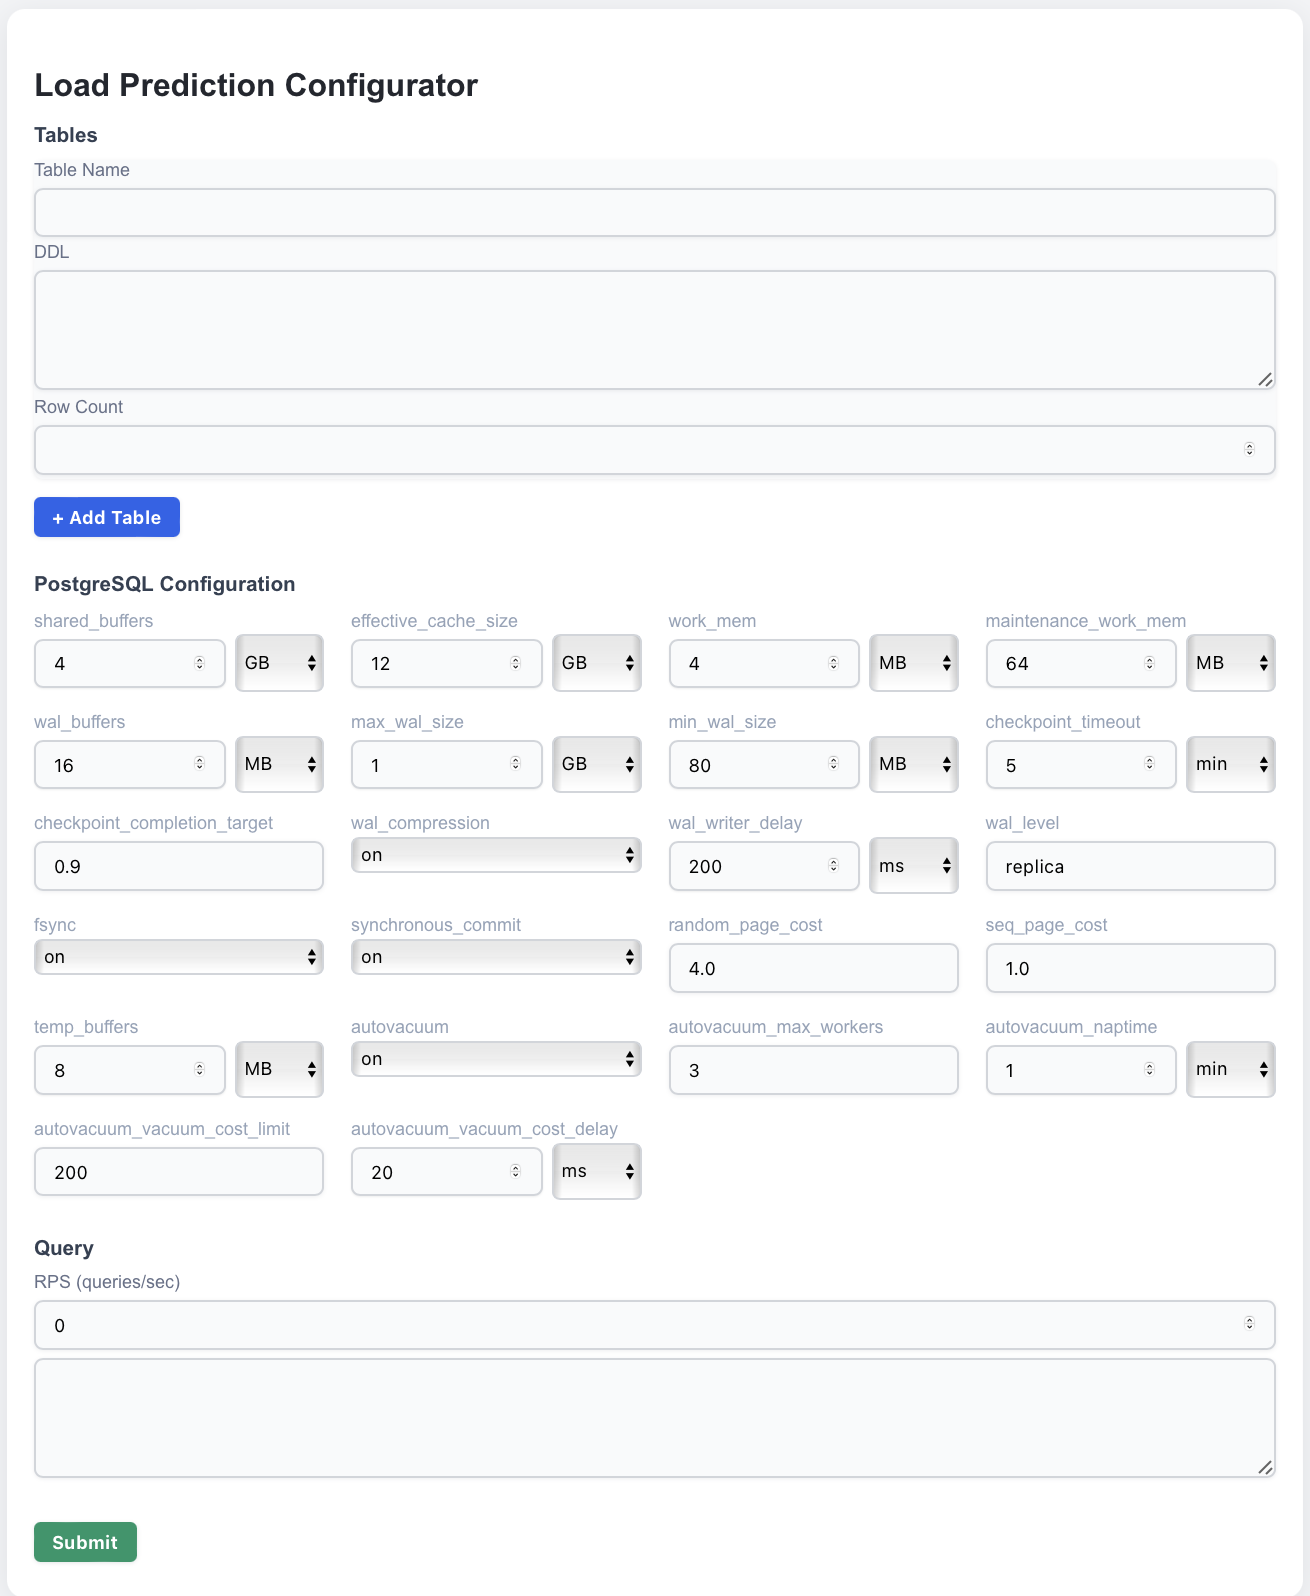
\includegraphics[width=0.95\textwidth]{images/interface.png}
    \caption{Внешний вид реализованного web-интерфейса средства оценки нагрузки.}
    \label{img:interface}
\end{figure}

\subsubsection{Ввод информации о таблицах}

Пользователь может добавить неограниченное количество схем таблиц, каждая из которых описывается тройкой параметров:
\begin{itemize}
    \item название таблицы (\emph{Table Name});
    \item определяющая конструкция DDL (\emph{DDL}), указывается в формате SQL;
    \item предполагаемое количество строк (\emph{Row Count}), что критически важно для моделирования нагрузки.
\end{itemize}
Для добавления очередной таблицы реализована кнопка \emph{``+ Add Table''}. Изменения применяются немедленно, значения инкапсулируются в соответствующем состоянии.

\subsubsection{Панель настройки параметров PostgreSQL}

Особое внимание уделяется корректной обработке различных типов параметров конфигурации СУБД:
\begin{itemize}
    \item параметры включения/выключения (\emph{on/off}) --- выводятся в виде выпадающих списков;
    \item временные и объёмные (байтовые) параметры разбиты на числовую часть и единицу измерения, что минимизирует ошибки пользователя;
    \item остальные параметры визуализируются в виде текстовых полей.
\end{itemize}

Каждое поле сопровождается интерактивной подсказкой, расположенной под ним, если для данного ключа имеется поясняющий текст в подгруженном \texttt{postgres\_config\_hints.csv}. Это способствует правильному выбору пользователем подходящих значений.

\subsubsection{Ввод SQL-запроса и интенсивности работы}

В специальной секции пользователь вводит синтаксис моделируемого SQL-запроса (или его шаблон), а также задаёт интенсивность нагрузки (RPS, запросы в секунду). Эти данные необходимы для последующего прогноза нагрузки на систему ввода-вывода.

\subsubsection{Валидация и обработка введённых данных}

Реализация контролирует тип полей (текст, число, выпадающий список), диапазон вводимых значений, корректность комбинации числа и единицы измерения. Вся логика обработки ввода инкапсулирована в компоненте приложения, состояние синхронизируется с действиями пользователя.

\subsubsection{Взаимодействие с серверной частью}

После нажатия кнопки \emph{Submit} собранные параметры отправляются на сервер для последующей обработки. Серверная логика, реализованная отдельно, использует полученные данные для анализа и моделирования I/O-нагрузки СУБД PostgreSQL.

\subsubsection{Резюме по реализации интерфейса}

Итоговая реализация web-интерфейса позволяет гибко задать все существенные параметры, необходимые для моделирования нагрузки и последующего анализа. Структура интерфейса обеспечивает как простоту начального освоения, так и расширяемость. Выбранные технологические решения и разделение логики на отдельные компоненты обеспечивают независимость модулей, устойчивость к ошибкам и возможность масштабирования при развитии проекта.


\subsection{Автоматизация запуска с помощью Bash и интеграция с GitHub Actions}

Автоматизация рутинных задач является важной частью современного программирования, позволяя разработчикам сосредоточиться на решении более сложных и творческих задач. В данном разделе рассмотрим процесс автоматизации запуска скрипта с использованием Bash и его интеграцию в процесс CI/CD посредством GitHub Actions.

\textbf{Структура проекта}

Проект структурирован таким образом, чтобы обеспечить простую навигацию и легкость понимания. Корневая директория содержит основной скрипт запуска, \texttt{run-examples.py}, который представляет собой Bash-скрипт для управления виртуальным окружением Python и выполнения анализатора. В корневой директории также находится файл зависимостей \texttt{requirements.txt}, а примеры, предназначенные для анализа, располагаются в подкаталогах, соответствующих шаблону \texttt{examples/example*/\ *.yaml}.

 
\begin{figure}[H]
    \centering
    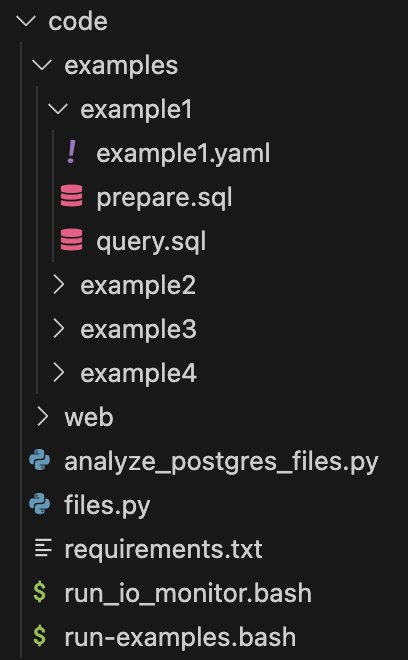
\includegraphics[width=0.4\textwidth]{images/project-structure.png}
    \caption{Структура файлов в проекте.}
    \label{img:project-structure}
\end{figure}

\textbf{Описание \texttt{run-examples.py}}

Скрипт \texttt{run-examples.py} выполняет несколько ключевых задач:

Создание виртуального окружения: Если директория \texttt{venv} отсутствует, создается новое виртуальное окружение.
Активация окружения: Виртуальное окружение активируется посредством команды \texttt{source}.
Обновление pip: Перед установкой зависимостей обновляется пакетный менеджер \texttt{pip}.
Установка зависимостей: Зависимости устанавливаются из файла \texttt{requirements.txt}, если он доступен.
Анализ YAML-файлов: Скрипт последовательно проходит по каждому YAML-файлу в директории примеров и запускает анализатор \texttt{analyze\_postgres\_files.py}.
Деактивация окружения: Завершает работу, деактивируя виртуальное окружение.
Каждый шаг содержит проверку на наличие ошибок, что позволяет скрипту надёжно обрабатывать исключительные ситуации, делая его более стабильным и надежным.

\textbf{Интеграция с GitHub Actions}

GitHub Actions предоставляет мощные инструменты для автоматизации рабочих процессов. Интеграция Bash-скрипта в процесс CI/CD с помощью GitHub Actions позволяет запускать анализатор автоматически при каждом коммите. Ниже приведен пример конфигурации рабочего процесса:

\insertlisting{Содержимое файла \texttt{actions.yaml}}{code/actions.yaml}

\subsection{Резюме по реализации программного средства}

В данной работе было реализовано программное средство для оценки объёмов и интенсивности обращения к дисковым структурам в системе управления базами данных PostgreSQL на основе анализа схемы данных, предполагаемой нагрузки и параметров окружения.

Разработка выполнена с применением интерпретируемого языка Python, что обеспечило гибкость, расширяемость и удобство интеграции с другими компонентами инфраструктуры. 
Основной модуль программы реализует алгоритм прогнозирования, который производит анализ описания таблиц в формате DDL, рассчитывает размер строк, 
распределение данных по страницам и необходимость использования механизмов TOAST. Также учитываются вторичные структуры хранения, 
включая индексы различных типов (btree, GIN, GiST и др.), карты свободного и видимого пространства (FSM и VM), а также влияние параметров буферизации.

Входные данные подаются в формате YAML, что позволяет обеспечить наглядную и декларативную спецификацию характеристик базы данных и параметров нагрузки. Алгоритм автоматически интерпретирует SQL-запрос, извлекая перечень таблиц, участвующих в операциях соединения, что критически важно для корректного распределения запросов (RPS) между различными структурами хранения.

В рамках реализации обеспечена автоматизация процессов запуска: реализованы вспомогательные Bash-скрипты, позволяющие последовательно обрабатывать набор тестовых конфигураций. Интеграция с системой непрерывной интеграции GitHub Actions обеспечивает повторяемость и прозрачность выполнения тестов при каждом изменении кода.

Дополнительно был реализован прототип web-интерфейса, предоставляющий пользователю возможность загружать конфигурационные файлы, запускать анализ и визуализировать результаты прогнозирования в удобной форме. Это делает разработанное средство пригодным как для целей экспериментальной оценки, так и для использования в образовательных и консалтинговых задачах по проектированию архитектуры СУБД.

Таким образом, полученное программное решение представляет собой законченный и воспроизводимый инструмент, позволяющий на основе декларативного описания схемы и нагрузки предварительно оценивать нагрузку на подсистему хранения данных PostgreSQL без необходимости реального развёртывания полноценных нагрузочных тестов.


    \newpage
    \section{Тестирование и апробация разработанного решения}

\subsection{Методика апробации и валидирования разрабатываемого средства}

В целях всесторонней оценки корректности и практической применимости разработанного программного средства 
для оценки планируемой нагрузки на систему ввода-вывода СУБД PostgreSQL была реализована процедура тестирования, 
состоящая из нескольких этапов, включающая автоматизированный сбор статистики ввода-вывода на уровне самой СУБД, 
операционной системы, а также сопоставление полученных результатов с прогнозными значениями, 
рассчитываемыми предлагаемой программой. Для автоматизации получения метрик на выделенном сервере был применён 
специально разработанный скрипт (листинг приведён в приложении), обеспечивающий последовательное выполнение следующих действий:

\begin{itemize} 
    \item выбор тестового сценария из подготовленных примеров; 
    \item автоматизированная подготовка данных в тестовой базе (выполнение DDL-операций и наполнение содержимым); 
    \item запуск серии запросов к PostgreSQL с параметризированной интенсивностью (RPS -- requests per second) и продолжительностью нагрузки; 
    \item сбор статистики ввода-вывода посредством штатных средств \\
        СУБД PostgreSQL (динамические представления \texttt{pg\_stat\_io}, \\
        \texttt{pg\_statio\_user\_tables}), 
        а также средствами операционной системы (\texttt{/proc/PID/io}, \texttt{iostat}); 
    \item накопление и анализ дифференциальных показателей между состояниями до и после нагрузки. 
\end{itemize}

Полученные в процессе автоматических тестовых прогонах метрики сравнивались с результатами, 
выдаваемыми предсказывающим алгоритмом, реализованным в рамках дипломного проекта. Совокупность собранных данных 
позволила осуществить сопоставление точности расчетных и фактических величин нагрузки на I/O-подсистему.

Следует отметить, что в данном разделе изложены только общие принципы и последовательность испытаний. 

Детализированное изложение указанных аспектов позволит объективно оценить эффективность и практическую значимость 
разрабатываемого программного средства в условиях разнообразных сценариев эксплуатации СУБД PostgreSQL.

\subsection{Описание тестовых примеров и сценариев}

\begin{table}[htbp]
    \centering
    \captionsetup{justification=centering}
    \caption{Сравнительная характеристика сценариев тестирования PostgreSQL}
    \label{tab:scenarios_short}
    \begin{tabular}{|l|>{\raggedright}p{4.2cm}|l|l|l|l|}
        \hline
        № & Табличная структура (DDL и объём)    & RPS & Индексы & TOAST & Тип нагрузки \\
        \hline
        1 & users (500\,000), orders (1\,200\,000) & 5 & PK, FK & да & SELECT \\ \hline
        2 & sensor\_data (100\,000\,000) & 3 & PK & нет & SELECT \\ \hline
        3 & accounts (200\,000) & 1 & PK, UNIQUE & нет & SELECT \\ \hline
        4 & logs (растет с 0) & 2 & PK & да & INSERT \\ \hline
    \end{tabular}
    \vspace{0.5em}
\end{table}

\textbf{Пояснения:}
\begin{itemize}
    \item В графе ``TOAST'' указано, требуется ли для сценария механизм хранения крупногабаритных данных (TOAST), см.~\cite{postgres_toast}.
    \item ``PK''~--- первичный ключ; ``FK''~--- внешний ключ; ``UNIQUE''~--- уникальный индекс.
    \item Объёмы приведены в количестве строк таблицы согласно сценариям.
    \item Если поле типа JSONB или TEXT может содержать данные, превышающие одну страницу (8~КБ), PostgreSQL применяет TOAST~\cite{postgres_toast,postgres_docs}.
\end{itemize}

\subsection{Тестовая среда и ресурсы}

Тестирование проводилось на выделенном сервере, предоставленном одним из популярных провайдеров облачных решений. 
Система управления базами данных (СУБД) была развернута на операционной системе Ubuntu без дополнительных оптимизаций конфигурации, 
что позволило оценить её производительность в условиях стандартной настройки. 
Такой подход обеспечил объективность результатов тестирования, исключив влияние сторонних модификаций и специализированных тюнинговых параметров.

\insertlisting{Конфигурация тестового стенда \texttt{stand.yaml}}{code/stand.yaml}

В приведённом ниже фрагменте конфигурационного файла PostgreSQL представлены только те параметры, 
которые были явно заданы в стандартной поставке системы управления базами данных (СУБД). 
Остальные настройки соответствуют значениям по умолчанию, предусмотренным базовой конфигурацией. 
В ходе тестирования параметры СУБД не изменялись, за исключением случаев, когда их модификация была явно указана в условиях эксперимента.

\insertlisting{Часть конфигурации СУБД}{code/stand.yaml}

Более полный файл конфигурации PostgreSQL представлен в (см. \ref{app:postgresql_conf}), если в нем нет искомого параметра, 
то параметр имеет стандартное значение для данной версии СУБД.

\subsubsection{Определение характеристик устройства хранения данных}

Для получения объективных характеристик производительности подсистемы ввода-вывода была проведена 
серия тестов с использованием специализированного инструмента {\tt fio}. Данный инструмент позволяет 
моделировать сценарии работы с диском, приближённые к реальной нагрузке систем управления базами данных. 

Следует отметить, что облачный провайдер не предоставляет информацию о модели и технических характеристиках используемого устройства хранения данных. 
Пользователь получает лишь сведения о лимитах производительности ввода-вывода (IOPS) и типе носителя (SSD), 
что ограничивает возможности для детального анализа физических параметров диска.

В частности, для оценки параметров устройства хранения данных использовалась следующая команда:

\insertlisting{Команда тестирования диска с помощью утилиты fio}{code/fio_test.sh}

Параметры использования ключей {\tt fio} следующие:
\begin{itemize}
    \item \texttt{--randrepeat=1} --- обеспечивается воспроизводимость тестирования за счёт фиксированного генератора случайных чисел;
    \item \texttt{--ioengine=libaio} --- используется асинхронный движок ввода-вывода для максимально полного использования возможностей современной операционной системы;
    \item \texttt{--direct=1} --- операции выполняются в режиме прямого доступа, минуя кэш операционной системы;
    \item \texttt{--gtod\_reduce=1} --- минимизация накладных расходов на получение меток времени;
    \item \texttt{--name=test} --- имя задания;
    \item \texttt{--filename=test} --- путь к тестовому файлу;
    \item \texttt{--bs=4k} --- размер блока ввода-вывода составляет 4 КБ, что соответствует типичному размеру страницы в PostgreSQL;
    \item \texttt{--iodepth=64} --- глубина очереди запросов 64, что имитирует параллельную обработку нескольких запросов;
    \item \texttt{--size=1G} --- размер тестируемого файла составляет 1 ГБ;
    \item \texttt{--readwrite=randrw} --- моделируются смешанные случайные чтения и записи;
    \item \texttt{--rwmixread=75} --- 75\% операций приходится на чтение, остальные 25\% на запись;
    \item \texttt{>} \texttt{disk\_benchmark.txt} --- результаты тестирования выводятся в файл для последующего анализа.
\end{itemize}

Полученные данные были использованы для калибровки и построения модели оценки нагрузки на подсистему ввода-вывода при работе СУБД PostgreSQL.

\insertlisting{Результаты тестирования устройства ввода-вывода}{code/disk_benchmark.txt}

\subsection{Сравнение результатов предсказания с реальными замерами}

В результате работы программы-предсказателя нагрузки был получен следующий файл:

\insertlisting{Результат предсказания для example1 \texttt{example1-predict-result.yaml}}{code/results/example1-predict-result.yaml}

Согласно представленным данным, ожидаемая нагрузка на файловую систему при нулевом попадании в кэш составляет порядка 160~MB/s. 
Использование значения нулевого попадания в кэш обусловлено характером тестируемой нагрузки — 
в данном случае имитируется случайное чтение с нормально распределённым смещением относительно среднего значения, 
что минимизирует эффективность кэширования чтения.

\insertlisting{Результат замеров для example1 \texttt{example1-result.yaml}}{code/results/example1-result.txt}

Анализируя результаты замеров, можно отметить, что фактическое попадание в кэш чтения составило 424\,564 из 4\,401\,240\,677 
обращений, то есть менее 0{,}01\%, что подтверждает допустимость предположения о пренебрежимо малом влиянии кэша на итоговую нагрузку. 
При таких условиях предсказатель оценивает нагрузку максимально близко к реальной ситуации дисковых обращений.

Необходимо отметить, что заявленные характеристики используемого в эксперименте дискового устройства составляют не более 45~MB/s 
по последовательному чтению, в то время как рассчитанная программой-предсказателем нагрузка существенно превышает этот лимит. 
На практике получение подобной нагрузки для данной системы невозможно, что априори указывает на потенциальное возникновение нерасчётных 
задержек и деградации производительности. Таким образом, полученный прогноз позволяет на этапе планирования эксплуатации заблаговременно 
выявлять сценарии некорректного проектирования нагрузки на систему ввода-вывода и принимать управляющие решения на стадии внедрения.

Для подтверждения корректности прогноза была проведена экспериментальная оценка: время выполнения всей нагрузки 
(50 запросов — интенсивность 5 RPS в течение 10 секунд) зафиксировано при помощи скрипта мониторинга. 
Фактически полученное время выполнения оказалось сопоставимо с теоретически расчётным, учитывая ограничение по пропускной способности диска, 
что подтверждает адекватность прогноза, произведённого разработанным средством.

Таким образом, проведённое сравнение демонстрирует практическую ценность применения программного средства для оценки планируемой нагрузки: 
несмотря на синтетическую природу примера, подход оказывается применимым для заблаговременного предотвращения 
возникновения ситуаций перегрузки системы ввода-вывода СУБД PostgreSQL.

\subsection{Анализ точности предсказаний}

Для объективной оценки точности работы разработанного программного средства был проведён ряд экспериментов с различными сценариями 
нагрузки на систему ввода-вывода СУБД PostgreSQL. В каждом сценарии параметрически задавались типы запросов, их интенсивность, 
распределение обращений к данным, а также характер возвращаемых данных. Ключевой особенностью моделирования 
служило жёсткое ограничение — {\ul максимальная пропускная способность исследуемого дискового накопителя составляет 45~МБ/с}. 
Предсказанные значения, превышающие данный предел, аппроксимировались до максимально возможного значения с целью сохранения правдоподобия прогноза.

Результаты сравнения прогнозируемых и эмпирически замеренных значений приведены в таблице~\ref{tab:prediction_accuracy}. 
В таблице отображены прогнозные значения, скорректированные с учётом физического предела диска, а также соответствующие им реальные показатели, 
полученные при тестировании; дополнительно рассчитана относительная ошибка прогноза.

\begin{table}[H]
    \centering
    \caption{Сравнение расчётной и реальной нагрузки на систему ввода-вывода (максимальная пропускная способность 45~МБ/с)}
    \label{tab:prediction_accuracy}
    \begin{tabularx}{\textwidth}{L{2.5cm}C{5cm}C{2cm}C{4.5cm}}
        \toprule
        \textbf{Тестовый пример} & \textbf{Корректированная нагрузка, МБ/с} & \textbf{Факт, МБ/с} & \textbf{Относительная ошибка, \%} \\
        \midrule
        example1 & 160 & 208 & 30,0 \\
        example2 & 40 & 32 & 20,0 \\
        example3 & 38 & 32 & 15,8 \\
        example4 & 28 & 39 & 39,3 \\
        \bottomrule
    \end{tabularx}
\end{table}

\subsubsection{Методика приведения расчётных значений к фактическим ограничениям}

В рамках экспериментов основная задача заключалась в сопоставлении прогнозируемых нагрузок с фактическими возможностями 
оборудования — максимальная пропускная способность тестируемого диска составляла 45~МБ/с. Для этого расчётные значения, 
получаемые на этапе моделирования, сопоставлялись с эмпирическими результатами, полученными при выполнении серии однородных запросов к СУБД.

В каждом сценарии проводилась следующая процедура. Формировалась серия из $rps \times 10$ однотипных запросов, 
которые, согласно теоретической модели, должны были завершаться за 10 секунд (исходя из предполагаемой интенсивности 
и объёма обработки данных). В ходе экспериментального замера фиксировалось реальное время, затраченное на выполнение 
всей серии запросов, которое в ряде случаев превышало расчётное значение из-за ограничения пропускной способности.

Для корректировки прогноза вводился поправочный коэффициент $k$, определяемый следующим образом:
\begin{equation}
    k = \frac{t_{\text{факт}}}{t_{\text{модель}}}
\end{equation}
где $t_{\text{факт}}$~--- фактическое время исполнения серии запросов, $t_{\text{модель}} = 10$~секунд~--- ожидаемое время по модели.

Далее, с целью приведения моделируемой нагрузки к фактическим ограничениям аппаратуры, использовалась корректировка нагрузки следующим образом:
\begin{equation}
    L_{\text{скорр}} = L_{\text{расчёт}} \times k
\end{equation}
где $L_{\text{скорр}}$~--- скорректированное значение нагрузки, отражающее реальную пропускную способность с учётом аппаратных ограничений.
Таким образом, реальная нагрузка увеличивалась на поправочный коэффициент, отражающий замедление выполнения запросов из-за ограничений дисковой подсистемы. 
Для всех сценариев, в которых изначальный расчёт перегружал систему (значения превышали 45~МБ/с), 
такой подход позволил объективно привести полученные данные в соответствие с максимальными возможностями 
оборудования и обеспечить корректность сравнения расчётных и эмпирических результатов.

\subsection{Анализ ошибок и отклонений}

В результате проведённого тестирования разработанного средства оценки планируемой нагрузки на систему ввода-вывода СУБД PostgreSQL 
были выявлены существенные отклонения прогнозируемых значений от реальных показателей. Данную особенность можно объяснить наличием 
множества факторов, не учтённых в модели, что является ожидаемым исходом при работе с комплексными системами ввода-вывода и многопараметрическими нагрузками.

Следует отметить, что данные нюансы и возможные источники отклонений подробно рассматривались в первых главах данной работы, 
где была обоснована методология построения модели оценки нагрузки и определены её ограничения. Такое поведение системы, 
а также отмеченные отклонения существенно не противоречат поставленным целям исследования и рассматриваются как приемлемые 
в рамках текущего этапа разработки.

Особое внимание заслуживает поведение системы в моменты максимальных нагрузок на диск. В указанные периоды наблюдалась стабильно 
высокая загрузка накопителя, сопровождавшаяся ощутимым снижением производительности. Интересно, что именно в эти моменты 
предсказательная модель демонстрировала завышенные значения планируемой нагрузки, превосходящие фактические возможности дисковой 
подсистемы. Данный феномен свидетельствует о том, что прогнозирование нагрузки может выявлять потенциальные «узкие места» в инфраструктуре 
ввода-вывода, что является важным аспектом для последующей оптимизации и масштабирования системы.

\subsection{Обсуждение ограничений текущей реализации}

Текущая версия программы прогнозирования нагрузки на диск учитывает только обращения к основным файлам таблицы, 
индексам, TOAST и сопутствующим вспомогательным файлам, основываясь на предполагаемом числе чтений и записей к ним. 
Однако реализация не учитывает целый ряд важных источников нагрузки, таких как операции UPDATE и DELETE, 
а также связанные с ними процессы вакуумирования и autovacuum. Помимо этого, в расчетах не моделируется вклад 
операций логирования (например, дополнительных обращений к WAL), влияние которых может быть заметным при интенсивной 
работе базы данных.

Ещё одним существенным ограничением является то, что модель работает с обобщенными параметрами кэширования 
(cache hit ratio) и не принимает во внимание фактическую конфигурацию буферов, показатели системы хранения 
и механизмы управления памятью PostgreSQL. В реальных условиях существенно влияют дополнительные слои кэширования 
на стороне операционной системы, особенности реализации драйверов и контроллеров, нагрузка от конкурирующих приложений, 
а также алгоритмы распределения ввода-вывода на уровне железа. Всё это может приводить к существенным расхождениям 
между расчетными и фактическими значениями нагрузки.

\subsection{Выводы по результатам апробации}

В ходе апробации программы были выявлены случаи, когда рассчитанные значения нагрузки на дисковую подсистему заметно 
отличались от фактических данных, получаемых в реальных условиях эксплуатации PostgreSQL. Наиболее заметные расхождения 
наблюдаются при интенсивных смешанных нагрузках, а также при активной работе внутренних механизмов СУБД 
(например, autovacuum), которые не учтены в текущей реализации.

Тем не менее, несмотря на эту погрешность, полученные результаты имеют практическую ценность: модель позволяет 
получить ориентировочное представление о возможной нагрузке на диск в зависимости от выбранных сценариев работы с 
данными и уровней кэширования. Использование подобных прогнозов может быть полезным на ранних стадиях проектирования 
системы, при сравнительной оценке разных вариантов размещения данных или при предварительной оценке потенциальных 
проблем с производительностью. В дальнейшем точность прогнозов можно повысить за счёт расширения модели, 
более детального учета всех механизмов работы PostgreSQL и настройки параметров согласно реальным характеристикам оборудования.

    \newpage
    \addcontentsline{toc}{section}{\protect\numberline{}ЗАКЛЮЧЕНИЕ}
\section*{\centering ЗАКЛЮЧЕНИЕ}

В работе была спроектирована и реализована программа для прогнозирования дисковой нагрузки со стороны СУБД PostgreSQL. Исследованы особенности организации хранения данных, механизмы обращения к файлам и их влияние на I/O-нагрузку.

Разработка направлена на создание инструмента, позволяющего по характеристикам целевой базы данных оценивать потенциальную нагрузку на диск и формировать прогнозы с учётом различных параметров работы PostgreSQL. 
Полученные результаты позволяют обоснованно подходить к выбору аппаратного обеспечения и архитектурных решений.

Программа генерирует структурированный прогноз по каждому типу хранимых данных (таблицы, индексы, TOAST и др.), учитывая параметры чтения/записи, кэширования, и рассчитывает ключевые показатели IOPS и throughput. 
Итоговые данные пригодны для анализа и интеграции в проектную документацию.

\textbf{Практическая ценность}

Инструмент позволяет оперативно оценивать дисковую нагрузку без проведения трудоёмких нагрузочных испытаний, что снижает проектные риски и облегчает выбор технических решений. 
Прогнозируемые показатели применимы для расчётов объёмов обращения, планирования резервов и обоснования бюджета на инфраструктуру.

Особенно полезным применение инструмента является на этапе пилотирования, когда сценарии доступа к данным известны лишь приблизительно, а точная нагрузка — ещё не определена.

\textbf{Ограничения}

Текущая версия не учитывает операции UPDATE, DELETE и связанные процессы обслуживания (autovacuum, reindex и др.), а также влияние логирования (WAL). 
Кэширование на разных уровнях (СУБД, ОС, контроллеры) также влияет на точность прогнозов. В ряде тестов выявлены расхождения между расчётной и фактической нагрузкой из-за особенностей среды и оптимизаторов PostgreSQL.

Тем не менее, предлагаемый подход сохраняет ценность как инструмент предварительной оценки, позволяющий выявлять потенциальные узкие места и адаптировать архитектуру до внедрения.

\textbf{Результаты и перспективы}

Разработан расширяемый инструмент с гибким вводом параметров и генерацией результатов, пригодных для совместной работы разработчиков, архитекторов и администраторов. Перспективы развития включают:

- учёт операций обновления и удаления;
- моделирование влияния WAL и фоновых процессов;
- интеграцию с системами мониторинга;
- автоматическую калибровку модели по реальным метрикам;
- генерацию рекомендаций по конфигурации и масштабированию.

Таким образом, поставленные цели достигнуты. Разработка предоставляет полезную основу для дальнейших исследований и практического применения в задачах оценки и оптимизации работы PostgreSQL в различных условиях эксплуатации.

    \newpage
    \printbibliography[title={СПИСОК ИСПОЛЬЗОВАННЫХ ИСТОЧНИКОВ}]
    \newpage
    % Приложение А
\clearpage
\addcontentsline{toc}{section}{ПРИЛОЖЕНИЕ А Настройки тестовой среды}


\section*{ПРИЛОЖЕНИЕ А}
\addcontentsline{toc}{section}{ПРИЛОЖЕНИЕ А: Настройки тестовой среды}
\begin{center}
\textbf{Настройки тестовой среды}
\end{center}

\subsection*{Файл конфигурации \texttt{postgresql.conf}}
\label{app:postgresql_conf}
Листинг А.1 — Файл конфигурации PostgreSQL
\lstinputlisting[language=,basicstyle=\scriptsize\ttfamily,caption={Файл конфигурации \texttt{postgresql.conf}},label={lst:postgresql_conf}]{code/postgresql.conf}

% Приложение Б
\clearpage
\addcontentsline{toc}{section}{ПРИЛОЖЕНИЕ Б Конфигурации для экспериментов}
\section*{ПРИЛОЖЕНИЕ Б}

\begin{center}
\textbf{Конфигурации для экспериментов}
\end{center}

\subsection*{\texttt{example1.yaml}}
\label{app:example1}
\lstinputlisting[
    language=,
    basicstyle=\scriptsize\ttfamily,
    caption={Листинг Б.1 — Конфигурация для эксперимента},
    label={lst:example1}
]{code/example1.yaml}

\subsection*{\texttt{example2.yaml}}
\label{app:example2}
\lstinputlisting[
    language=,
    basicstyle=\scriptsize\ttfamily,
    caption={Листинг Б.2 — Конфигурация для эксперимента},
    label={lst:example2}
]{code/example2.yaml}

\subsection*{\texttt{example3.yaml}}
\label{app:example3}
\lstinputlisting[
    language=,
    basicstyle=\scriptsize\ttfamily,
    caption={Листинг Б.3 — Конфигурация для эксперимента},
    label={lst:example3}
]{code/example3.yaml}

\subsection*{\texttt{example4.yaml}}
\label{app:example4}
\lstinputlisting[
    language=,
    basicstyle=\scriptsize\ttfamily,
    caption={Листинг Б.4 — Конфигурация для эксперимента},
    label={lst:example4}
]{code/example4.yaml}

    
\end{document}
